\customsection{Diseño del sistema}
\subsection{Diseño conceptual}
Como primera medida se deicidio diseñar el sistema con 2 programas (escritorio y celular) que fueran capaces de acceder a la base de datos directamente, porque resultaba ser la topología más sencilla para lograr los requerimientos funcionales. El diagrama de bloques del concepto se puede observar en la figura \ref{primier_diagramaGeneralizado}. Teniendo en cuenta la figura \ref{primier_diagramaGeneralizado}, los bloques azules representan objetos de importancia para la comprensión del flujo de la información en el sistema, los bloques grises representan rutinas importantes de los objetos anteriormente mencionados y los bloques naranjas son directamente la interfaz de comunicacion con el servidor. En el diagrama se puede observar como se planeó tener la comunicacion con el servidor MySql directamente a través de sus Apis. También, se puede ver como la relación Raspberry y celular es de generador y vizualizador, es decir, que con esta topología no se podía controlar la vivienda de manera remota.
\vspace{0.5cm}\\

\begin{figure}[htbp]
	\centering
	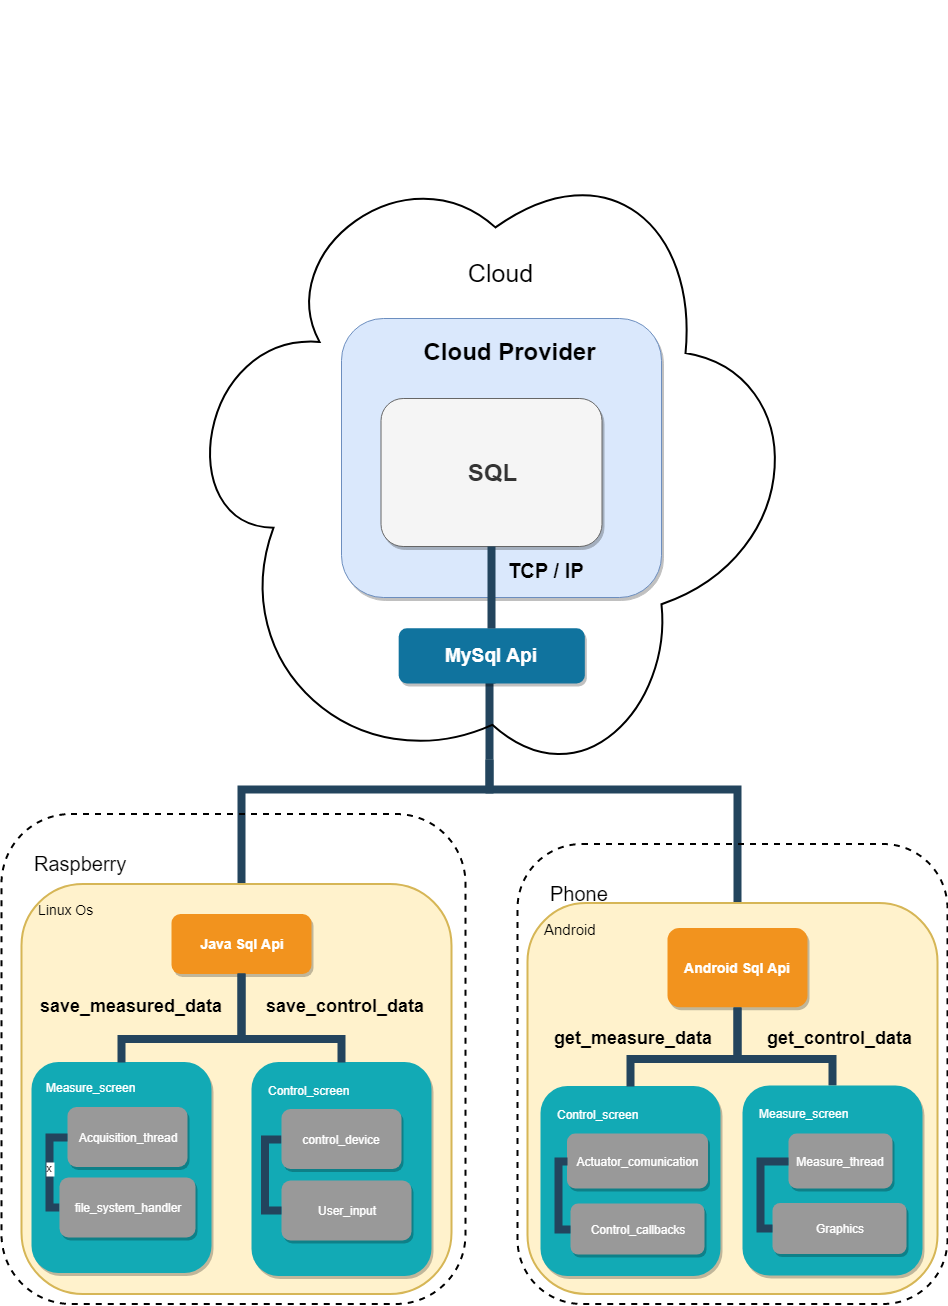
\includegraphics[width=15cm]{figuras/first_GeneralDiagram.png}
	\caption{Primer diseño generalizado de la estructura del sistema Fuente: propia}	
	\label{primier_diagramaGeneralizado}
\end{figure}

Durante el proceso de implementación se cambió el diseño a una topología con mas seguridad y escalabilidad, esto debido a que la anterior topología permitía el acceso directo de los programas cliente a la base de datos, exponiéndola a brechas de seguridad.

\subsection{Diseño final}
El diseño final contemplo las mejores condiciones de: modularidad, costo, tamaño y escalabilidad. Para cada uno de estas características se escogieron tecnologías y se desarrollaron funciones claves. 
\vspace{0.5cm}\\
Desde la perspectiva de la modularidad, se diseñaron aplicaciones de \textit{frontend} capaces de integrar 2 tipos de protocolos de comunicación: Mqtts y Https; además, para acceder a los servicios de la nube se seleccionó el proveedor de servicios de backend ``Google Cloud Plataform'' puesto que permitirá utilizar de la mejor manera todos los servicios de Google: su asistente de voz, su interfaz de inteligencia artificial, sus servicios de autenticación, su red privada de fibra óptica (que es de las más rápidas y de mayor cobertura), entre otros. Una comparación mas a fondo de sus competidores y los motivos de esta selección se puede observar en el capitulo ``Serverless backend''.
\vspace{0.5cm}\\
En cuanto al costo, se utilizaron tecnologías de \textit{backend} totalmente escalables tipo \textit{serverless} para ajustar los gastos a únicamente los necesarios, teniendo en cuenta que las pruebas a gran escala estuvieron lejos del alcance de este proyecto, aún así se desarrolló toda la arquitectura pensando en la necesidad de optimizar en la mayor medida los gastos. Teniendo en cuenta que no se hicieron pruebas a gran escala los servicios de \textit{backend} fueron posibles gracias a las cuotas gratuitas del mayorista utilizado para desplegar el servicio (Google).
\vspace{0.5cm}\\
En cuanto al requerimiento de escalabilidad, la decisión de diseñar serverless jugó el papel más importante: Los servicios servirles le permitieron a la aplicación ser diseñada para permanecer funcional sin hacer ningún cambio inclusive con 4000 dispositivos conectados (esta última apreciación es teórica puesto que no se hicieron pruebas a esa escala).
\vspace{0.5cm}\\
El producto del \textit{backend} se diseño para utilizar el servicio de Google Cloud y utilizó los siguientes elementos para su funcionamiento: Un ``Google Cloud Storage Bucket'' conectado a la red privada de Google para el almacenamiento de archivos, Una base de datos relacional MySql para el almacenamiento de datos de monitoreo y control de los dispositivos, una lista de ``funciones de nube''  activadas por solicitudes Https y por ellas mismas que se comunican directamente con la base de datos y finalmente, un \textit{broker} nativo de Google Cloud llamado ``Cloud IOT'' que recibe las conexiones de Mqtts de los dispositivos del sistema.
\vspace{0.5cm}\\
La aplicación móvil se diseñó para estar compuesta de 3 escenas: la escena de control, utilizada para el manejo de los actuadores disponibles desde el aplicativo en sitio; la escena de medición, encargada de presentarle al usuario las mediciones adquiridas por el aplicativo en sitio en tiempo real; y la escena principal, donde se puede observar un indicador del porcentaje de las variables mas relevantes respecto a un punto de referencia. Por ejemplo, el porcentaje de consumo de agua con respecto al promedio de consumo de agua en un mes de un grupo familiar.
\vspace{0.5cm}\\
Finalmente, el aplicativo en sitio se diseñó para manejar un flujo de datos más grandes y la posibilidad de funcionar desconectado de la red. La aplicación se diseño para permitirle al usuario programar rutinas de control de los circuitos a partir de horarios, visualizar los datos medidos, cambiar parámetros de adquisición como el tamaño del \textit{buffer} y la frecuencia de muestreo, entre otros.
\vspace{0.5cm}\\
Para comprender mejor el diseño, se puede observar en la figura \ref{diagramaGeneralizado} un diagrama generalizado de los componentes de software del sistema, donde principalmente los desarrollos hacen parte de 3 grandes bloques: el bloque de la nube, el bloque del dispositivo embebido (Raspberry), y el bloque del dispositivo móvil (Android).
\vspace{0.5cm}\\
\begin{figure}[htbp]
	\centering
	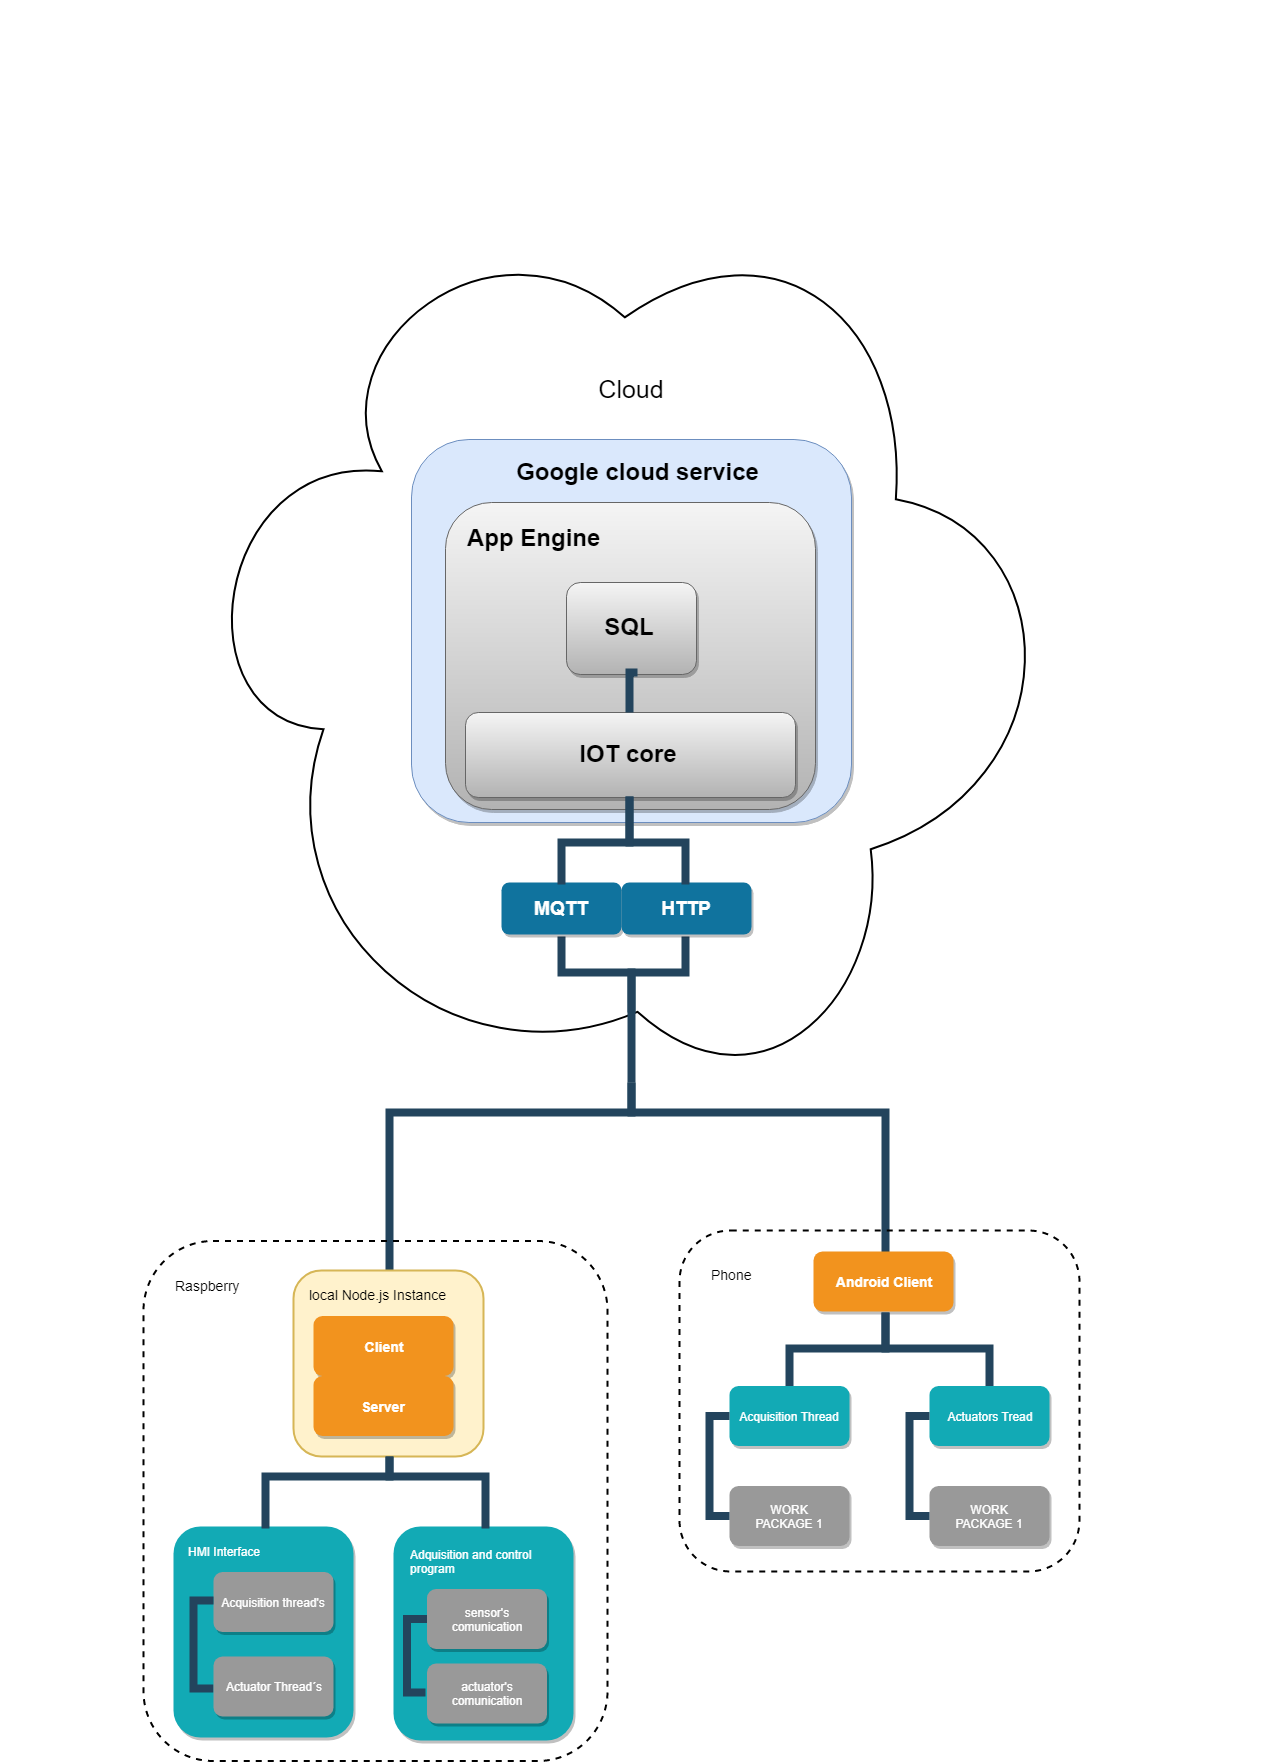
\includegraphics[width=15cm]{figuras/GeneralDiagram.png}
	\caption{Diagrama generalizado de las entidades software del proyecto. Fuente: propia}	
	\label{diagramaGeneralizado}
\end{figure}
En el nuevo diseño de programa se puede observar como la comunicación con el \textit{backend} esta gobernada por el protocolo Mqtts desde la perspectiva de la aplicación de escritorio; para esto se utiliza el cliente de Mqtts de Python. Por otro lado, la comunicación del cliente móvil esta gobernada por el cliente Fetch de Javascript. Otro cambio importante del diseño del sistema, es que en la ventana de control se eliminó el componente de visualización del estado actual de control, y se cambio por un generador de mensajes de control a travéz de solicitudes Https tipo Post. Teniendo en cuenta lo anterior, se añadió una rutina de atención de eventos de control, provenientes del \textit{backend}. Es decir que, ahora la aplicación de escritorio podría recibir ordenes de control desde la aplicación celular.
\vspace{0.5cm}\\
El flujo de la información del diagrama generalizado se puede observar en el diagrama de secuencia de la figura \ref{secuencia}. En el diagrama se observan los eventos y las funciones más importantes involucradas en el proceso de comunicacion entre aplicaciones.
\begin{figure}[htbp]
	\centering
	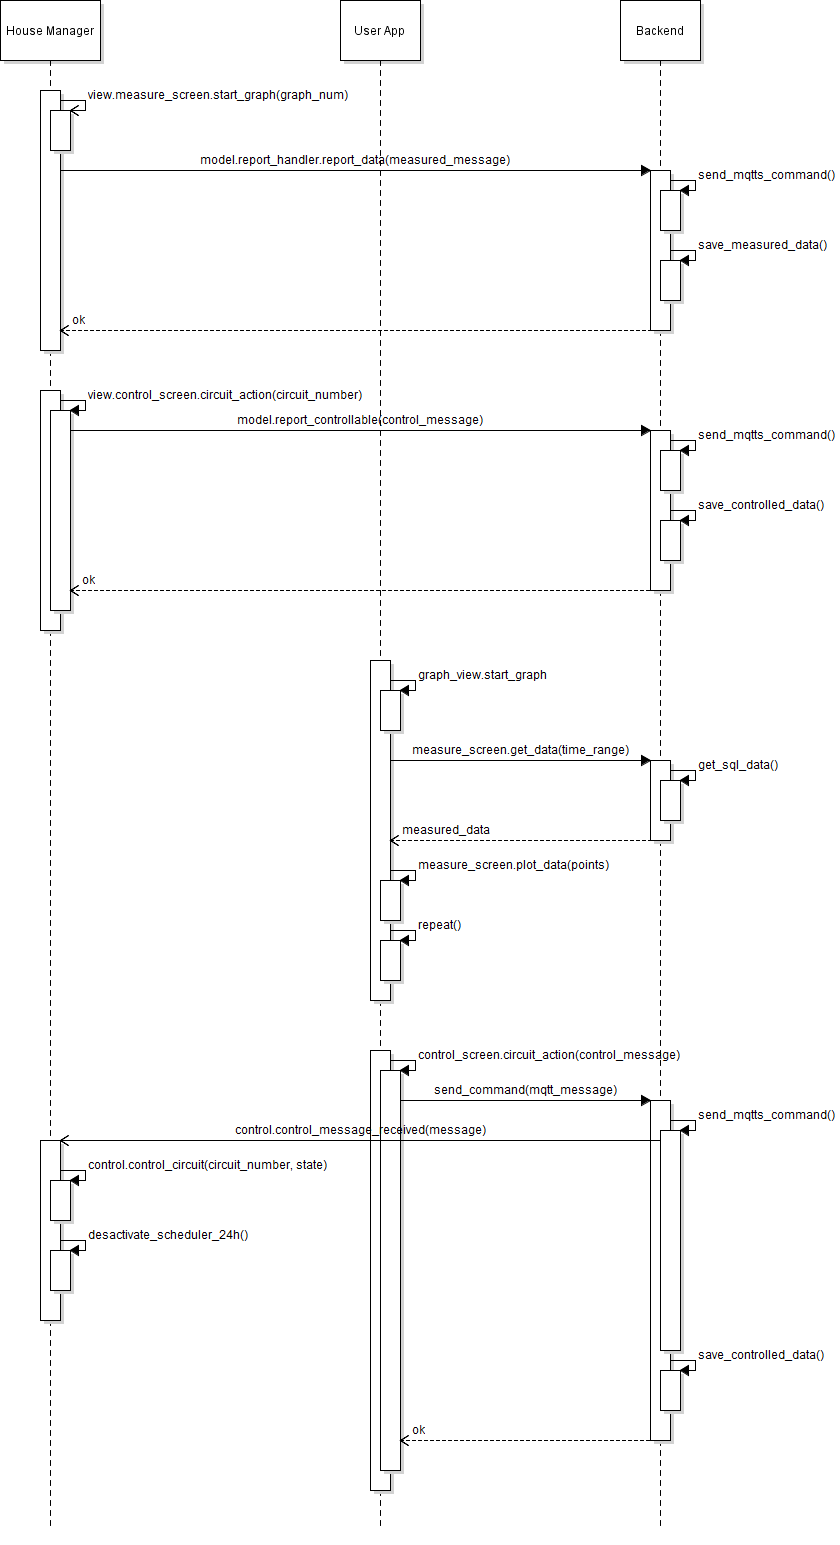
\includegraphics[width=11cm]{figuras/secuencia.png}
	\caption{Diagrama de secuencia general de la comunicación. Fuente: propia}	
	\label{secuencia}
\end{figure}
